\documentclass[12pt]{article}

\usepackage{amsmath, color}
\usepackage{mdwmath}
\usepackage{amssymb, epsf, epsfig, textcomp}
\renewcommand{\baselinestretch}{0.9}
\usepackage{a4wide}
\newcommand{\argmin}{\mathop{\mathrm{argmin}}}
\usepackage{caption}
\usepackage{subcaption}
\usepackage{mathtools}
\usepackage{listings}
\lstdefinestyle{myCustomMatlabStyle}{
	basicstyle=\ttfamily\footnotesize,
	breaklines=true,
	language=Matlab,
	numbers=left,
	stepnumber=1,
	numbersep=10pt,
	tabsize=4,
	showspaces=false,
	showstringspaces=false
}
\begin{document}
	\begin{center}
		{\bf Reinforcement Learning and Dynamic Optimization} \\
		Assignment 2: Experts and Adversarial Bandits\\%(120/1000) \\
		Report Delivery Date: Friday, April 28, 2023 \\
	\end{center}
	{\bf Student: }Alevrakis Dimitrios 2017030001\\
	
	\begin{enumerate}
		\item []{\bf Assignment Description} \\
		We are given a dataset of real traffic loads over time (normalized), for a number of servers. These demands are non stationary. The dataset was given in csv file
		
		The goal is to devise algorithms that learn to predict the least loaded server at every time round. Imagine, for example, that you had to offload computing tasks, one after another, to one of these servers: the higher the load of the server at that time, the longer the delay for your own offloaded task as well.
		
		\item[{\bf Part I}]
		We implement the Multiplicate Weights algorithm assuming an experts or a bandits environment.
		
		Following the suggestions of the uploaded lecture notes the parameters chosen where:\\
		For the Experts environment:
		\begin{align}
			\eta = \sqrt{\frac{lnk}{T}}
		\end{align}
		
		and for the Bandits environment:
		\begin{align}
			\eta = \epsilon = \sqrt[3]{\frac{lnk}{T}}
		\end{align}
		
		
		Comparison of the cumulative regret of each algorithm, for horizon values $T=1000,7000$.
		\begin{figure}[h!]
			\centering
			\begin{subfigure}[b]{0.45\textwidth}
				\centering
				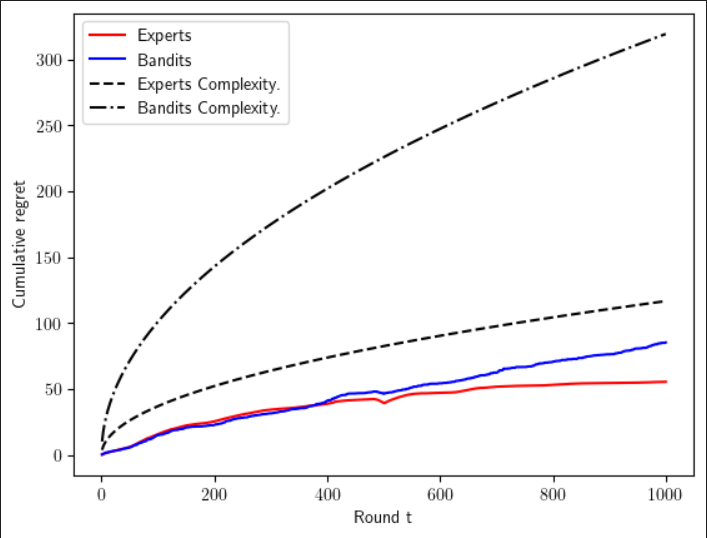
\includegraphics[width=\textwidth]{fig1.png}
				\caption{$T=1000$}
			\end{subfigure}
			\hfill
			\begin{subfigure}[b]{0.45\textwidth}
				\centering
				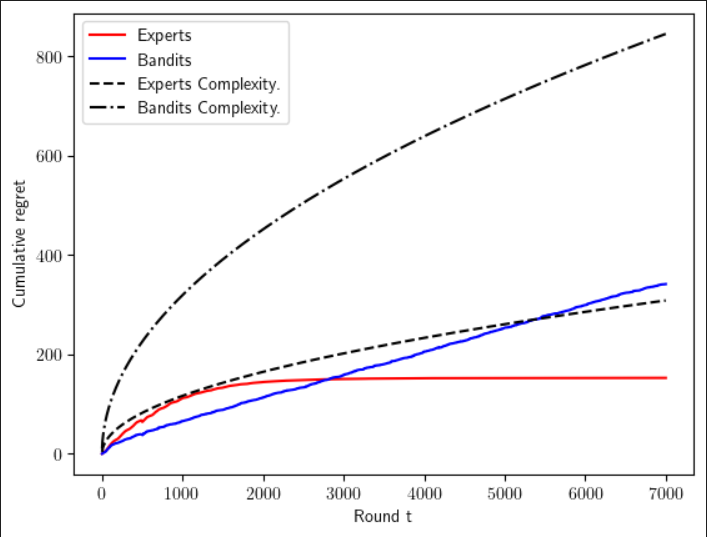
\includegraphics[width=\textwidth]{fig2.png}
				\caption{$T=7000$}
			\end{subfigure}		
		\end{figure}
	
		\newpage
		By observing the graphs we can see that that in both cases the algorithm achieve a Regret lower than their upper bounds. We can also observe that while for a lower horizon the two algorithms have comparable performance. Although for a bigger horizon the hostile environment of the bandits algorithm is made obvious by its significantly worse performance than the experts algorithm.\\
		
		The respective algorithm upper bounds:
		\begin{itemize}
			\item Experts: $O(2\sqrt{tlogk})$
			\item Bandits: $O(\sqrt{tklogk})$
		\end{itemize}
		\item[{\bf Part II}]
		We adapt the UCB algorithm to the above problem.\\
		In order for the  algorithm to be adapted we consider the reward as the loss and calculating $ucb_i=-\mu_i + \sqrt{\frac{lnT}{Q_i(t)}}$ in order to choose the arm yielding the lower loss or the arm chosen the least.
		\begin{figure}[h!]
			\centering
			\begin{subfigure}[b]{0.45\textwidth}
				\centering
				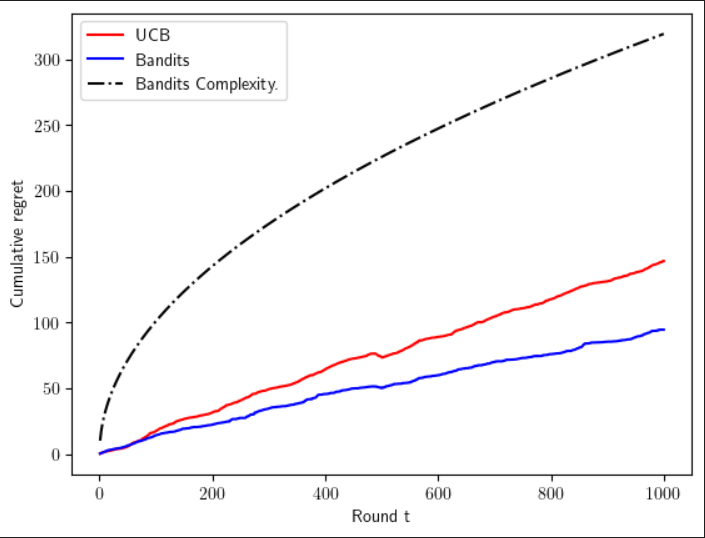
\includegraphics[width=\textwidth]{fig3.png}
				\caption{$T=1000$}
			\end{subfigure}
			\hfill
			\begin{subfigure}[b]{0.45\textwidth}
				\centering
				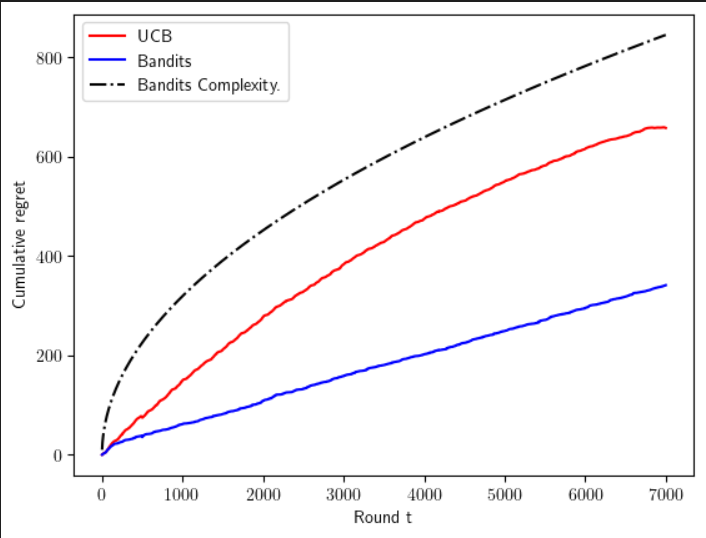
\includegraphics[width=\textwidth]{fig4.png}
				\caption{$T=7000$}
			\end{subfigure}		
		\end{figure}
	
		Since the UCB algorithm is deterministic it fails in a bandit environment thus performing worse than the bandit algorithm.
	\end{enumerate}
	
\end{document}
